\documentclass[twocolumn,conference]{article}

\usepackage{amsmath,amssymb,amsfonts}
\usepackage{xcolor}
\usepackage{listings}
\usepackage{inputenc}
\usepackage{graphicx}
\usepackage{authblk}
\usepackage{enumerate}
\usepackage{caption}

\usepackage{array,booktabs,longtable,tabularx}
\usepackage{ltablex}
\usepackage{wrapfig,lipsum,booktabs}
\usepackage{multirow}

\providecommand{\keywords}[1]
{
  \small	
  \textbf{\textit{Keywords---}} #1
}

\begin{document}
\author[1]{Eric Raphael Huiza Pereyra}
\affil[1]{Artificial Intelligence Research Group (IAPUCP) - Post Graduate Program - Pontificia Universidad Católica del Perú}
\affil[]{\textit{eric.huiza@pucp.edu.pe}}

\author[2]{Cesar Armando Beltrán Castañon}
\affil[2]{IA-PUCP}
\affil[]{\textit{cbeltran@pucp.edu.pe}}

\title{%
	\vspace{-2.0cm}
	\textbf{Talking with signs} \\	
	\Large \textbf{A self supervised method to detect nouns and numbers in a non-annotated signs language corpus}
}

\maketitle
    
\begin{abstract}
Self supervised learning is a current topic that allows transferring learned latent variables on pre-text tasks into downstream tasks achieving notable increases in terms of model performance. In this work we present a self supervised approach for learning latent variables in a non annotated Peruvian Signs Language dataset using a SwAV based approach applied to video datasets. We present a novel signs detection model (nSDmV3) which takes advantage of a pre-trained self supervised features detection model. obtaining XX\% AUC To our knowledge it is the first work that uses SwAV as a baseline to detect signs in a non-annotated dataset. 
\\
\keywords{self supervised learning, SwAV, latent variables,Peruvian signs language}
\end{abstract}
\section{Introduction}\label{Introduction}
Starting a model architecture design by considering the usage of pre-trained models is always a good starting point,  even when using a ResNet50 network backbone pre-trained with ImageNet the resulting model will leverage a set of fine tuned layers decreasing hours and data volume required for training. There have been some efforts to build an annotated Peruvian Signs Language (PSL) dataset (Bejarano et al) with promising but still small results. In this paper we are using Self Supervised techniques to overcome the current low annotated PSL dataset availability problems towards to obtain improved results of a previous work that was focused on Supervised learning and classic movement and pattern recognition techniques \cite{Pereyra_2021_CVPR}.  

Signs languages can be described from spatial-temporal features extracted from isolated glosses and a large set of continuous streams of contextually related frames.  Similar to other languages, context is extremely important to define what is semantically correct and to provide meaning to a set of interconnected glosses which relations can easily become extremely complex and can only be described from an also extremely large set of spatial and temporal features but most importantly latent variables intrinsic to the data. 

This work is focused on non contrastive clustered methods in order to decrease the computation needed to compare feature by feature required for constrastive methods. Our method is based on Swapping Assignments between multiple Views (SwAV) \cite{caron2020unsupervised} as a backbone and extended it to design a set of model architectures that can learn latent variables from a set of non annotated PSL videos, training our model with the PSL dataset generated by the department of grammar at PUCP.

Sign Language corpus annotation is a tedious and complex task where a set of automatic and manual tasks need to be orchestrated together in order to produce a quality corpus with statistical value. In this work we solve the problem of lack of annotated PSL datasets availability by proposing a self supervised method where a features detection model can be trained to learn latent variables while solving a set of pre-task in our case finding compatible augmented video fragments across the dataset in order to solve a downstream nouns and numbers classification task.

Finally we extended model architectures that were previously created as part of \cite{Pereyra_2021_CVPR} to use our SwAV based pre-trained model as a backbone and to improve the AUC of PR metric in these models. This work is divided on Related Work \ref{related-work},  Experimentation \ref{experimentation},  Discussion \ref{discussion} and Conclusion \ref{conclusion}

\section{Related Work}\label{related-work}
\subsection{Self Supervised Learning}
Predicting the future or reconstructing the past is a way to learn and understanding the hidden patterns and distributions in data which is not necessarily annotated or pre-processed. Schmidhuber proposed an early self supervised method \cite{schmidhuber1990making} where two fully self supervised recurrent neural networks predicted future reinforcement based on external interactions and state sent to the next network cell is calculated on differences on successive predictions achieving a system capable to generate supervision signals. Unlike supervised tasks where predictions are influenced by target and observed variables, self supervised tasks are influenced in a greater extent by hidden or invisible variables also known as latent variables. By capturing those dependencies, a model can be used to answer questions about the values of unknown variables given the values of known variables. Energy-Based Models (EBMs) capture dependencies by associating a scalar energy (a measure of compatibility) to each configuration of the variables. Inference, i.e., making a prediction or decision, consists in setting the value of observed variables and finding values of the remaining variables that minimize the energy. Learning consists in finding an energy function that associates low energies to correct values of the remaining variables, and higher energies to incorrect values. A loss functional, minimized during learning, is used to measure the quality of the available energy functions. Within this common inference/learning framework, the wide choice of energy functions and loss functionals allows for the design of many types of statistical models, both probabilistic and non-probabilistic \cite{lecun2006tutorial}.

Unsupervised visual representation learning, or self-supervised learning, aims at obtaining features without using manual annotations and is rapidly closing the performance gap with supervised pre- training in computer vision. Many recent state-of-the-art methods build upon the instance discrimination task that considers each image of the dataset (or “instance”) and its transformations as a separate class. This task yields representations that are able to discriminate between different images, while achieving some invariance (latent variables) to image transformations. Recent self-supervised methods that use instance discrimination rely on a combination of two elements: a contrastive loss and a set of image transformations. The contrastive loss removes the notion of instance classes by directly comparing image features while the image transformations define the invariances encoded in the features. Both elements are essential to the quality of the resulting networks \cite{caron2020unsupervised}. Caron et al 2020 proposed a cluster based (non constrastive or architectural) approach for learning latent variables or invariance from non annotated datasets that is extendable to video datasets called SwAV (Swapping Assignments between views). SwAV uses an online clustering mechanism that is capable to scale well to large datasets including video by solving an optimal transport problem using the Sinkhorn distance. 

\subsection{Signs Language Recognition and annotation}
Signs Language Recognition (SLR) are roughly divided in two categories Isolated SLR and Continuous SLR\cite{adaloglou2020comprehensive}.

\subsubsection{Isolated Signs Language Recognition}
Methods using this approach will assume individual and well defined glosses that are recognized in a series of video frames. Recognizing gestures is a difficult task, due to intrapersonal and interpersonal variations in performing them. In \cite{kennaway2015avatar} a new descriptive language called SiGML (Signing Gesture Markup Language) is presented, SiGML was developed from HamNoSys, the Hamburg Notation System. HamNoSys is a notation for recording sign language gestures, developed by researchers on sign language at the IDGS (Institut für Deutsche Ge-bädensprache) at the University of Hamburg, it is not specific to any one sign language, but is intended to cover all signing gestures in all sign languages. It records sign languages elements in terms of hand shape, hand location and hand movement and other special terms for non manual gestures. Signs are not holistic gestures but are rather analyzable, as a combination of linguistically significant features. Similarly to spoken languages, Signs Languages are composed of the following indivisible features\cite{adaloglou2020comprehensive}:
\begin{itemize}
\item Manual features, i.e. hand shape, position, movement, orientation of the palm or fingers
\item Non-manual features, namely eye gaze, head-nods/ shakes, shoulder orientations, various kinds of facial expression as mouthing and mouth gestures.
\end{itemize}
SiGML provides a formal notation that is easily understood by computer because it is XML based.

\subsubsection{Continuous Signs Language Recognition}
Continuous Signs Language Recognition (CSLR) uses contextual information that is not limited to spatial information that resides around the hand shape for fixed point in time, but also temporal information that consists of hand and body movements. Signs are famously multi-channel, information is carried in the hand shape, motions, body pose and even facial gestures \cite{slimane2021context}, \cite{camgoz2017subunets}. While models that recognize text based language use punctuation marks to separate sentences, CSLR models use pauses e.g. silent regions. There have been studies in the literature addressing automatic sign segmentation. However to the best of the authors’ knowledge, there is no study which utilizes sign segmentation for realizing continuous sign language recognition for complex scenarios. Following successful segmentation, the system needs to under-stand what information is being conveyed within a sign sentence. Current approaches tackle this by recognizing sign glosses and other linguistic components. Such methods can be grouped under the banner of CSLR. From a computer vision perspective, this is the most challenging task. Considering the input of the system is high dimensional spatio-temporal data, i.e. sign videos, models are required that understand what a signer looks like and how they interact and move within their 3D signing space. Moreover, the model needs to comprehend what these aspects mean in combination. This complex modeling problem is exacerbated by the asynchronous multi-articulatory nature of sign languages. Although there have been promising results towards CSLR, the state-of-the-art can only recognize sign glosses and operate within a limited domain of discourse, namely weather forecasts \cite{camgoz2020sign}

\subsubsection{Sign Languages Recognition Approaches}
\textbf{Specialized sub-networks (SubUNets)} allow decomposing a complex signs recognition problem into a series of specialized expert systems allowing to learn both spatial and temporal features where each subunit learns an intermediate representation that is transferred to the next subunit. (Camgoz et al.) \cite{camgoz2017subunets} proposed an architecture where each SubUNet consists of three tiers, firstly Convolutional Neural Network layer to learn spatial features, then a Bidirectional Long Short Term Memory layer to learn temporal features on top of the spatial features and finally a Connectionist Temporal Classification Loos layer to allow the networks to be trained with different length videos and label sequences. (Huang et al.) \cite{huang2018videobased} proposed a two streams \textbf{3DCNN} architecture for learning global (entire video frame) and local (hands area crop) video representations in combination with a Hierarchical Attention Network (HAN) for latent space based recognition eliminating the need for temporal layers as proposed in other studies \cite{slimane2021context}, \cite{camgoz2017subunets}, \cite{camgoz2020sign}. HAN is an extension of LSTM which incorporates the attention mechanism based on the structure of input. It uses a latent space which maps video representations learned on the 3DCNN streams with relevant video sentences using one hot encoding vectors. The encoder in the HAN reflects the hierarchical structures in its inputs and incorporates the attention mechanism.
\section{Experimentation}\label{experimentation}
Our proposed self supervised signs detection approach is composed mainly for two well defined processes, a self supervised training architecture based on SwAV and a classifier that takes takes advantage of transfer learning from a fined tuned features detector from the first one.  
The dataset is a set of non annotated videos that were recorded in different sessions where twenty four signers were interviewed with the same or similar questionary. Videos in their raw format are processed through a data ingestion pipeline which converts videos in a single continuous video stream which is then passed through our self supervised architecture based in SwAV but adapted for videos using a SubUNet type of architecture. After training our self supervised system we obtained a features detector that learned latent variables from the dataset in a self supervised fashion. Finally used the features detector as a backbone model in our nSDmV3 classifier.
\subsection{Self Supervised Training}\label{self-supervised-training}
Our method uses a Multi Crop input data pipeline which receives a continuous video stream and produces augmented video fragments using a set of data augmentation transformations as described in \ref{multi-crop-data-pipeline}. We configured the input data pipeline to produce video fragments where frames were cropped in 224x224 and 96x96, in our experimentation each training step receives five video fragment transformations, two 224x224 and three 96x96.
Our self supervised training architecture uses a features detection model (nSDmV3 Features Detection Model) based on SubUNet where augmented video fragments are inputs of a RRN using LSTM cells where each frame is an input of a RestNet50 backbone to ensure learning spatial and temporal features and representing these features in a video embedding vector. These embedding vectors are then used as inputs of a Projections Model that follows a fully-connected architecture composed of two dense layers a batch normalization layer, and two dense layers. The entire self supervised training architecture is described on Figure \ref{fig:nsdmv3-self-supervised-training-model-architecture}

\begin{figure*}[hbt!]
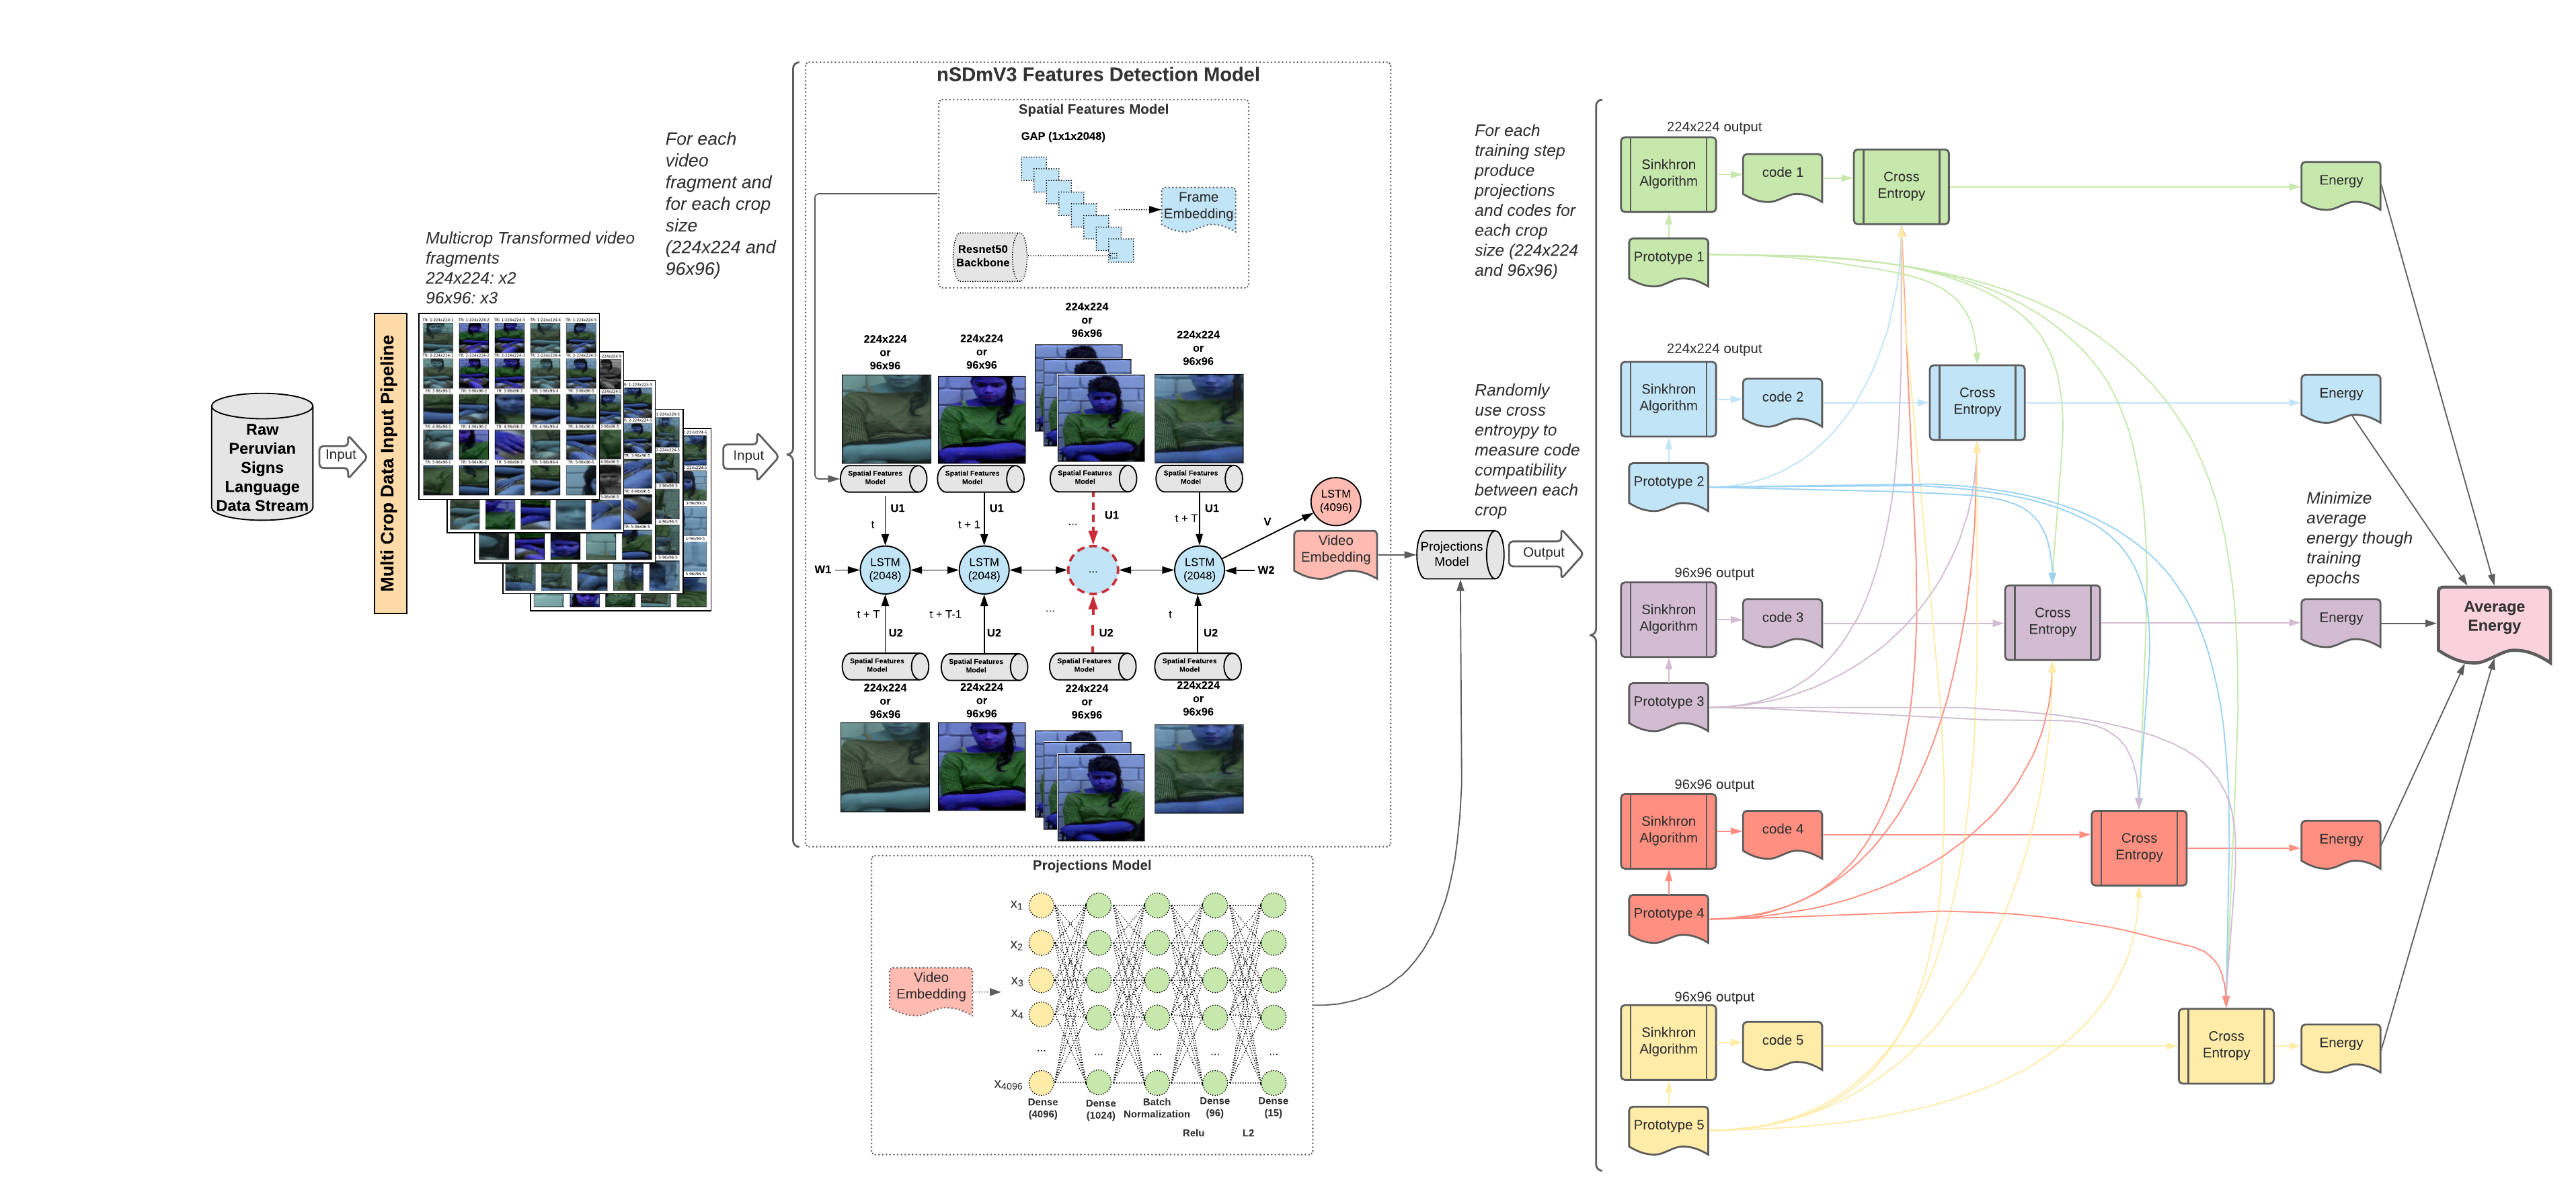
\includegraphics[width=\textwidth,height=\textheight,keepaspectratio]{images/nsdmv3-self-supervised-training-model-architecture.png}
\caption{nSDmV3 Self Supervised Training}
\label{fig:nsdmv3-self-supervised-training-model-architecture}
\end{figure*}

The projection model maps video embedding vectors to a set of clusters or prototype vectors which are then coded using the Sinkhron Algorithm to ensure a balanced vector codification. Codes and prototype vectors are then contrasted using cross entropy where one video video augmentation code is contrasted with all other video augmentation prototypes looking for compatibility towards to learn latent variables within the dataset. Finally the energy produced by each energy function in this case the cross contrasting using cross entropy is averaged with the objective to minimize the average energy across the training epochs.

\subsubsection{Multicrop Data Pipeline}\label{multi-crop-data-pipeline}
Our data input pipeline receives raw formatted videos and converts them in a continuous video stream using a \textbf{Video Stream Generator} component. Video steams are then sent to a \textbf{Data Preparer} component which is responsible to produce random duration video fragments between 0.5 and 1.5 seconds. A Human Detection Model is used to detect humans on video fragment frames getting rid of frame areas that will not contribute to learning PSL elements.

Video Fragments frames are randomly cropped using a 224x224 high resolution crops and 96x96 low resolution crops. Crops are then augmented in a sequence of transformations (Gaussian Blur, Color Jitter, Color Drop and Flip Left to Right).  Figure \ref{fig:nsdmv3-multicrop-data-pipeline-architecture} present architecture details.

\begin{figure*}[hbt!]
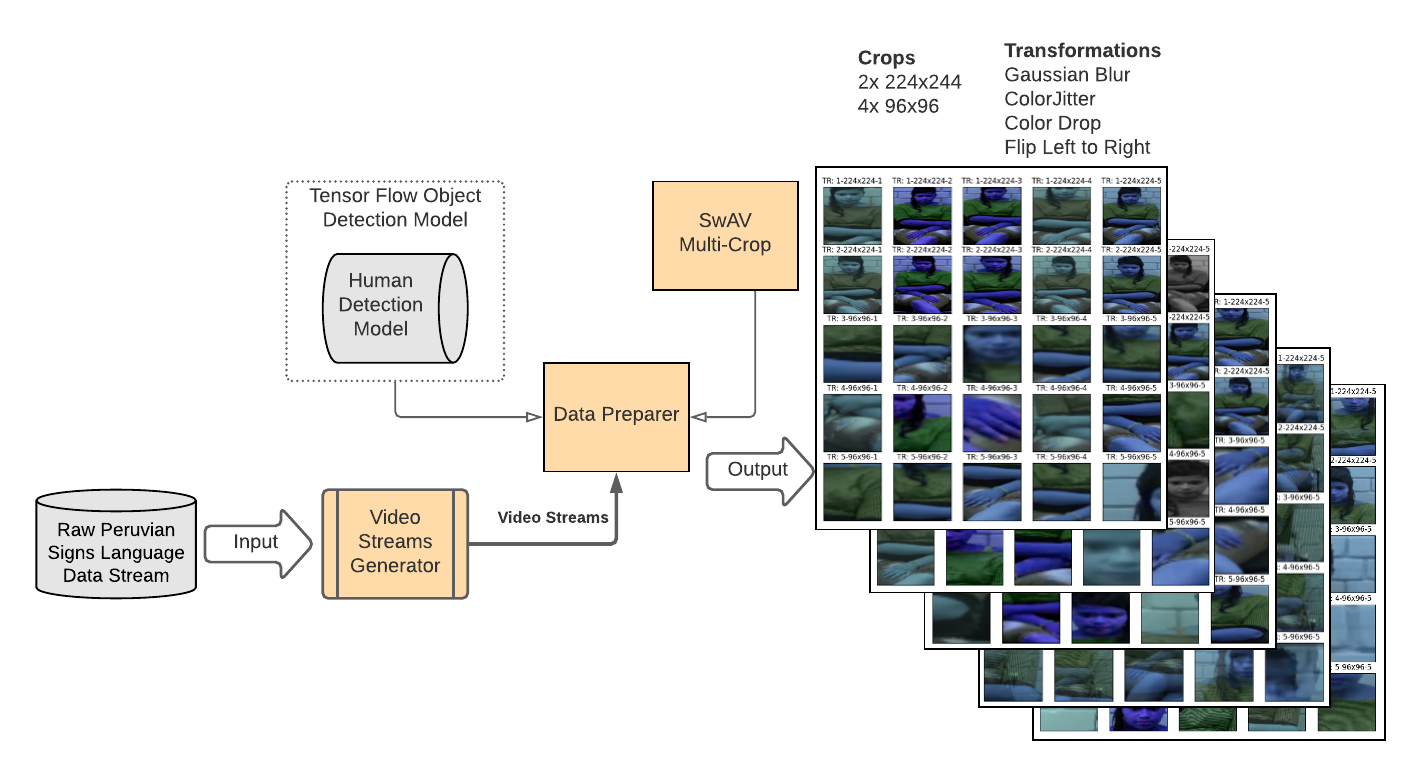
\includegraphics[width=\textwidth,height=\textheight,keepaspectratio]{images/nsdmv3-self-supervised-training-data-input-architecture.png}
\caption{nSDmV3 Multicrop Data Pipeline Architecture}
\label{fig:nsdmv3-multicrop-data-pipeline-architecture}
\end{figure*}

\subsection{nSDmV3 Classifier}\label{nsdmv3-classifier}
We evolved a previous signs detection model architecture nSDmV2 as described on \cite{Pereyra_2021_CVPR} into a novel architecture that uses the Features Detection Model defined on \ref{fig:nsdmv3-self-supervised-training-model-architecture} as a backbone with all its layer fine tuned. The features detection backbone is concatenated with fully-connected layers using dense, batch normalization layers and finally a dense layer with a softmax activation. nSDmV3 classifier architecture is described in Figure \ref{fig:nsdmv3-classifier-architecture} 

\begin{figure*}[hbt!]
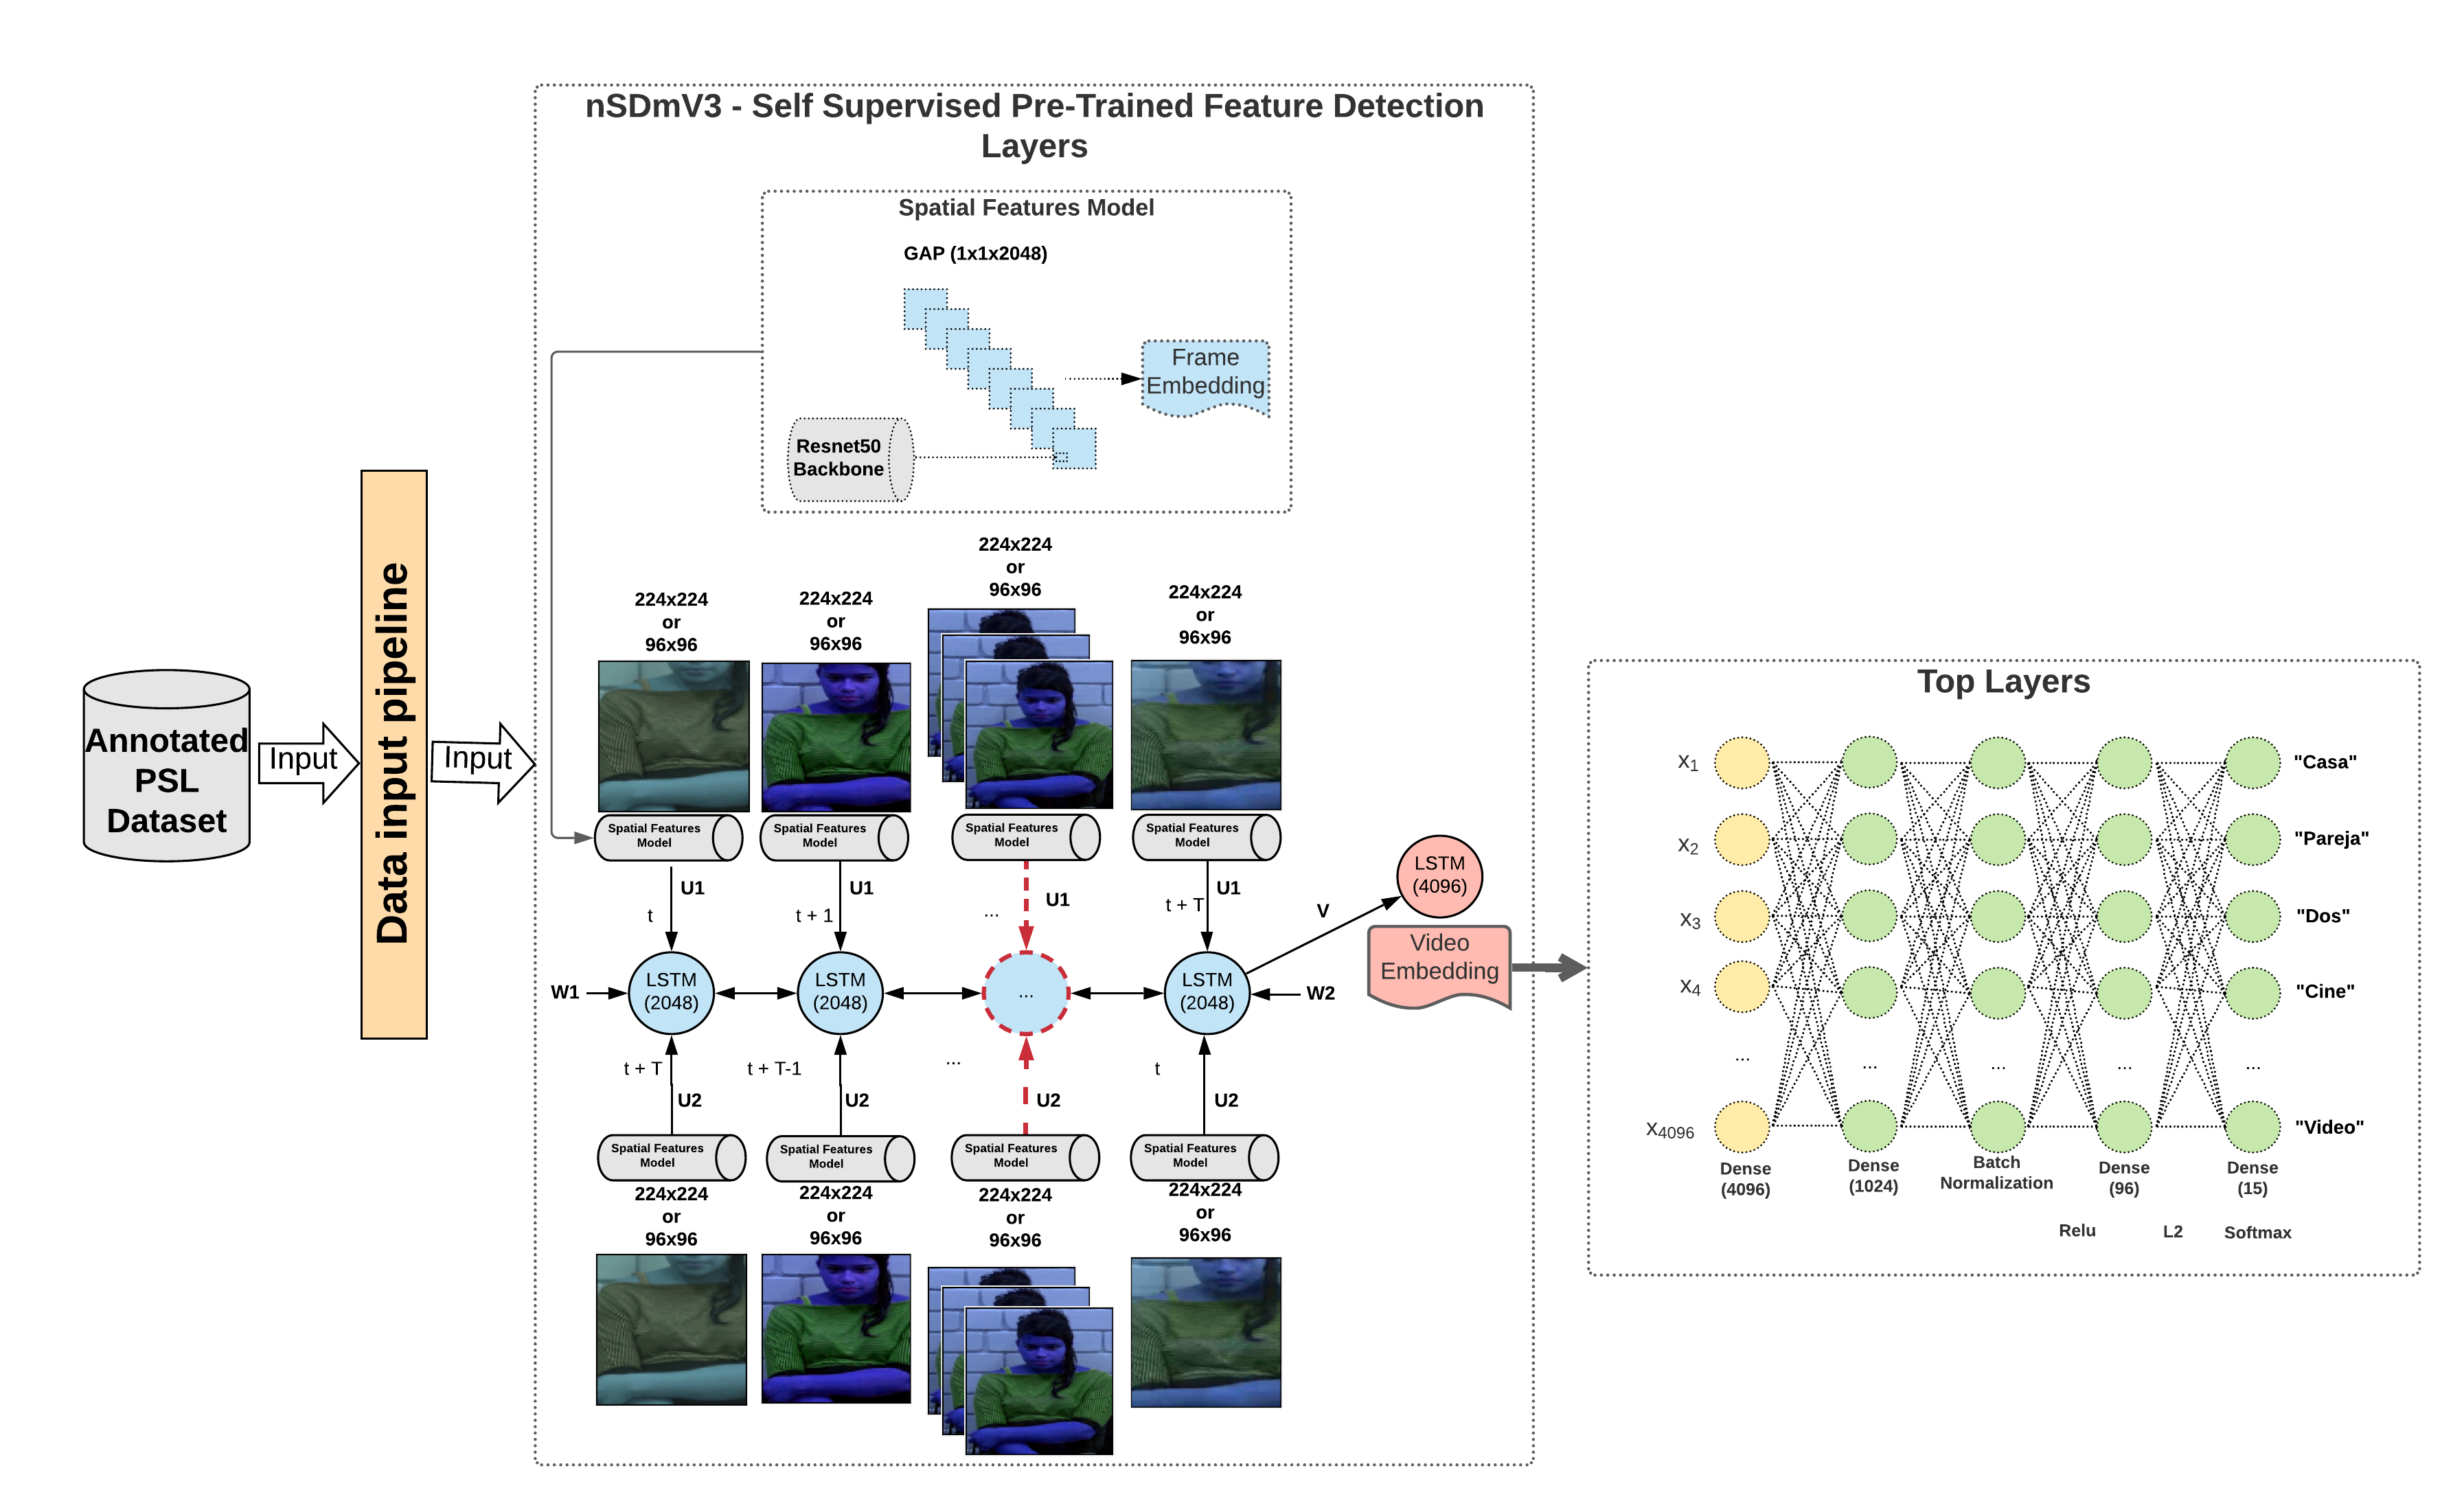
\includegraphics[width=\textwidth,height=\textheight,keepaspectratio]{images/nsdmv3-classifier-architecture.png}
\caption{nSDmV3 Classifier Architecture}
\label{fig:nsdmv3-classifier-architecture}
\end{figure*}

\subsection{Results}\label{results}
Our proposed self supervised architecture goal is to achieve successful metrics with a small number of annotated samples. The results presented on tables \ref{tab:nSDmV2-detection-results-5-percent} and \ref{tab:nSDmV3-detection-results-5-percent} indicate an increase on Precision, Recall and AUC on nSDmV3 compared to nSDmV2.

% nSDmV2 5% of the dataset
\begin{table*}
\captionsetup{font=footnotesize}
\centering
\begin{tabular}{ p{2.8cm} p{2.8cm} p{2.8cm} p{2.8cm} p{2.8cm} }
\toprule
\multicolumn{5}{c}{\textbf{nSDmV2 Training Results with the 5\% of the dataset}} \\
\hline
\hline
\textbf{Epoch}&	\textbf{Loss}	&\textbf{Precision}	&\textbf{Recall}	&\textbf{AUC} \\
\hline
\midrule
Epoch 1&	2.7568&	0.0000e+00&	0.0000e+00&	0.0911\\
Epoch 2&	2.6647&	0.0000e+00&	0.0000e+00&	0.1008\\
Epoch 3&	2.6455&	0.0000e+00&	0.0000e+00&	0.1017\\
Epoch 4&	2.6296&	0.0000e+00&	0.0000e+00&	0.1193\\
Epoch 5&	2.6121&	0.0000e+00&	0.0000e+00&	0.1222\\
Epoch 6&	2.6032&	0.0000e+00&	0.0000e+00&	0.1222\\
Epoch 7&	2.5943&	0.0000e+00&	0.0000e+00&	0.1229\\
Epoch 8&	2.5875&	0.0000e+00&	0.0000e+00&	0.1229\\
Epoch 9&	2.5825&	0.0000e+00&	0.0000e+00&	0.1229\\
Epoch 10&	2.5790&	0.0000e+00&	0.0000e+00&	0.1229\\
\bottomrule
\end{tabular}
\caption{Shows results of training the nSDmV2 model with the 5\% of the labeled PSL dataset: (1)\textit{Epoch} identifies the epoch in in the training process (2)\textit{Loss} obtained loss (3)\textit{Precision} obtained precision (4)\textit{Recall} obtained recall (5)\textit{AUC} area under the precision-recall curve.}
\label{tab:nSDmV2-detection-results-5-percent}
\end{table*}

% nSDmV3 5% of the dataset
\begin{table*}
\captionsetup{font=footnotesize}
\centering
\begin{tabular}{ p{2.8cm} p{2.8cm} p{2.8cm} p{2.8cm} p{2.8cm} }
\toprule
\multicolumn{5}{c}{\textbf{nSDmV3 Test Results with the 5\% of the dataset}} \\
\hline
\hline
\textbf{Epoch}&	\textbf{Loss}	&\textbf{Precision}	&\textbf{Recall}	&\textbf{AUC} \\
\hline
\midrule
Epoch 1&	X.XXXX&	X.XXXX&	X.XXXX&	X.XXXX\\
Epoch 2&	X.XXXX&	X.XXXX&	X.XXXX&	X.XXXX\\
Epoch 3&	X.XXXX&	X.XXXX&	X.XXXX&	X.XXXX\\
Epoch 4&	X.XXXX&	X.XXXX&	X.XXXX&	X.XXXX\\
Epoch 5&	X.XXXX&	X.XXXX&	X.XXXX&	X.XXXX\\
Epoch 6&	X.XXXX&	X.XXXX&	X.XXXX&	X.XXXX\\
Epoch 7&	X.XXXX&	X.XXXX&	X.XXXX&	X.XXXX\\
Epoch 8&	X.XXXX&	X.XXXX&	X.XXXX&	X.XXXX\\
Epoch 9&	X.XXXX&	X.XXXX&	X.XXXX&	X.XXXX\\
Epoch 10&	X.XXXX&	X.XXXX&	X.XXXX&	X.XXXX\\
\bottomrule
\end{tabular}
\caption{Shows results of testing the nSDmV3 model with the 5\% of the labeled PSL dataset: (1)\textit{Epoch} identifies the epoch in in the training process (2)\textit{Loss} obtained loss (3)\textit{Precision} obtained precision (4)\textit{Recall} obtained recall (5)\textit{AUC} area under the precision-recall curve.}
\label{tab:nSDmV3-detection-results-5-percent}
\end{table*}

\section{Discussion}\label{discussion}
It is possible to decrease and at some sort eliminate the need to annotate a dataset when pre-training a classifier features detection model using self-supervised techniques.  Our method approaches this problem using a SwAV based method towards to obtain a pre-trained features detection model trained with the PSL dataset leaning to a learn contextual and continuous patterns within the dataset. A classifier that use the pre-trained features detection model as a backbone is expected to have an boost on its performance in terms of AUC leaning to more simplistic and lighter video pre-processing and annotation tasks.

\section{Conclusion}\label{conclusion}
Self supervised techniques used to learn features from a non-annotated dataset stimulates and boosts positively the learning process by enabling the learning of latent variables in a non-annotated dataset. Pre-text tasks such us our SwAV based self supervised training pipeline is capable to extract and learn hidden features from the PSL dataset improving the AUC from our nSDmV3 classifier with respect to the previous version nSDmV2 in XX\%, obtaining a XX\% in comparison to the XX\% obtained with nSDmV2. The process to annotate a signs language dataset is tedious and complex requiring a great amount of manual annotation work along with a set of semi-automated pre-processing tasks. Self supervised techniques helps to decrease the amount of dataset annotation achieving successful results with low annotation levels. nSDmV3 along with our self supervised trainign pipeline are generalizable to other video related downstream tasks for the benefit of the scientific community.

\bibliographystyle{ieeetr}
\bibliography{References}

\end{document}
